\documentclass[sigconf]{acmart}

%% \BibTeX command to typeset BibTeX logo in the docs
\AtBeginDocument{%
  \providecommand\BibTeX{{%
    \normalfont B\kern-0.5em{\scshape i\kern-0.25em b}\kern-0.8em\TeX}}}

%% Remove ACM info
\settopmatter{printacmref=false}
\setcopyright{none}
\renewcommand\footnotetextcopyrightpermission[1]{}
\pagestyle{plain}

%%%%%%%%%%%%%%%%%%%%%%%%%%%%%%%%%%%%
% ----------- Packages ----------- %
%%%%%%%%%%%%%%%%%%%%%%%%%%%%%%%%%%%%
\usepackage{xspace}
%\usepackage[table,xcdraw]{xcolor}
\usepackage[inline]{enumitem}
%\usepackage[]{algorithm2e}
\usepackage{ifthen}
\usepackage{fancyhdr}
\usepackage{comment}
\usepackage[normalem]{ulem}
\usepackage{float}
\usepackage{placeins}
\usepackage{amsfonts}
\usepackage{amsmath}
\usepackage{amsthm}
\usepackage{verbatim}
\usepackage{graphicx}
\usepackage{algcompatible}
\usepackage{algorithm}
\usepackage{algpseudocode}
\usepackage{listings}
\usepackage{url}
\usepackage{hyperref}
\usepackage{threeparttable}
\usepackage{textcase}
\usepackage{minted}
\usepackage{etoolbox}

\usepackage{bigstrut}
\usepackage{booktabs}
\usepackage{tabularx}

\usepackage{lmodern}

\usepackage{tikz}
\usetikzlibrary{shapes.geometric, arrows, arrows.meta}
\usepackage{lipsum,adjustbox}

\usepackage{multirow}

\usepackage{blindtext}
\usepackage{scrextend}

%%%%%%%%%%%%%%%%%%%%%%%%%%%%%%%%%%%%
% ----------- Theorems ----------- %
%%%%%%%%%%%%%%%%%%%%%%%%%%%%%%%%%%%%
\newtheorem{remark}{Remark}
\newtheorem{example}{Example}
\newtheorem{pilotStudy}{Pilot Study}
\newtheorem{theorem}{Theorem}[section]
\newtheorem{definition}{Definition}
\newtheorem{corollary}{Corollary}[theorem]
\newtheorem{lemma}[theorem]{Lemma}

%%%%%%%%%%%%%%%%%%%%%%%%%%%%%%%%%%%%
% ------ Basic editorial format ------ %
%%%%%%%%%%%%%%%%%%%%%%%%%%%%%%%%%%%%
\newcommand{\ie}{{\it i.e.,}\xspace} 
\newcommand{\eg}{{\it e.g.,}\xspace} 
\newcommand{\Eg}{{\it E.g.,}\xspace} 
\newcommand{\etal}{{\it et al.}\xspace} 
\renewcommand{\sectionautorefname}{Section}
\def\definitionautorefname{Definition}

\BeforeBeginEnvironment{minted}{\vskip 10pt}
\AfterEndEnvironment{minted}{\vskip 10pt}


\begin{document}

%%%%%%%%%%%%%%%%%%%%%%%%%%%%%%%%%%%%
% ------ Paper Info ------ %
%%%%%%%%%%%%%%%%%%%%%%%%%%%%%%%%%%%%
\title{A Knowledge Graph Approach to Software Code Smells Detection in Python}

\author{By Yunfan Yang}
\author{Supervised by Jon Rokne}
 \affiliation{%
   \institution{University of Calgary}
   \city{Calgary}
   \state{AB}
   \country{Canada}
 }

% \author[1]{Author One}
% \author[2]{Author Two}

% \affil[1]{Department of Computer Science, University One}
% \affil[2]{Department of Physics, University Two}

% \affil[1]{\textit{author1@email.com}}
% \affil[2]{\textit{author2@email.com}}

\begin{abstract}
In the rapidly evolving landscape of software development, maintaining code quality is paramount. This paper introduces an innovative approach for detecting software code smells in Python. We propose a novel methodology for code analysis that leverages knowledge graphs, a powerful tool for representing and analyzing data relationships, for identifying and classifying code smells. The approach transcends traditional static analysis by integrating semantic understanding of code, thereby enhancing the detection of subtle yet critical anomalies that are often overlooked. Through rigorous evaluation on diverse Python codebases, the approach's efficacy in accurately identifying code smells is demonstrated, thereby contributing to improved code development, maintainability and reduced technical debt. This research provides a new direction in the application of knowledge graphs for software quality assurance.
\end{abstract}

\maketitle


% TikZ Presets
\tikzstyle{component} = [rectangle, minimum width=3cm, minimum height=1.2cm, align=center, text centered, draw=black, fill=cyan!20]
\tikzstyle{library} = [rectangle, minimum width=2cm, minimum height=0.8cm, align=center, text centered, draw=black, fill=yellow!20]
\tikzstyle{database} = [rectangle, minimum width=2cm, minimum height=0.8cm, align=center, text centered, draw=black, fill=orange!20]
\tikzstyle{intermediate} = [rectangle, minimum width=1.4cm, minimum height=0.8cm, align=center, text centered, draw=black, fill=red!20]

\tikzstyle{arrow} = [thick,->,>=stealth]
\tikzstyle{on arrow}=[fill=white, inner sep=2pt, midway, align=center, font=\scriptsize]

\tikzstyle{driver} = [rectangle, rounded corners, minimum width=2cm, minimum height=0.8cm, align=center, text centered, draw=black, fill=magenta!20]
\tikzstyle{flow} = [->, thick, magenta, shorten >=1pt]



% Separate LaTeX file for each section.  Please keep the filenames as they are unless discussed with other authors
\section{Introduction}
\label{sec:intro}


% Motivation
Today's software landscape is marked by escalating code complexity due to rising demands for software features. According to McKinsey's research, “software complexity grew by a factor of 4.0 over the past ten years, while 
software-development productivity increased by only a factor of 1.0 to 1.5. Today's average car contains more than 100,000 million lines of code" \cite{Burkacky_Deichmann_Frank_Hepp_Rocha_2021}. Furthermore, the integration of software components is also increasing. These factors increased the importance of detection and refactoring bad code which also remain vital for software analysis. Therefore, there is an urgent need for solutions to root out bad code.



% Background
"Bad smells" in code, often referred to as "code smells," are certain patterns in software development that suggest a deeper problem in the code. They are not bugs — code with smells usually functions correctly — but they indicate weaknesses that can slow down development or increase the risk of bugs or failures in the future.

A typical example of a code smell is \textit{Duplicated Code} \cite{Martin_2018}. This occurs when the same, or very similar, code exists in more than one location within a codebase. While duplicating code might seem a quick solution for a pressing problem, it can make maintenance and future changes challenging, as each instance of the duplication requires careful scrutiny to ensure consistency and correctness. Identifying and addressing such duplications is crucial for improving code quality and maintainability \cite{Martin_2018}.

Many studies have been done previously aims to detect code smells, with a significant number employing machine learning, deep learning, and even convolutional neural networks. In these past efforts, detection was largely driven by models trained for the task. Yet, the effectiveness of these models is greatly influenced by the organization of their training datasets, and consequently, they may underperform on certain codebases, undermining their perceived efficiency \cite{Nucci_Dario_Palomba_2018}. Prior research in this area has often overlooked the intricacies and challenges associated with large-scale software projects. Many of these studies have not delved deeply into the complexities that these larger projects introduce. As a result, the applicability and efficacy of predictive models become constrained when faced with detection tasks in such expansive software environments. This limitation highlights the need for more comprehensive studies and models tailored to address the unique characteristics with regards to code quality when faced with large-scale software projects \cite{Menshawy_Yousef_2021}.



% Problem Description

The problem is, therefore, to provide an improved solution to the problem of rooting out bad code in software since the currently available solutions are not providing adequate solutions.

Knowledge Graphs (KGs), as a powerful data graph representation of the real world knowledge, represent a transformative approach in the context of data analysis and information management. These graphs are increasingly recognized in the field of artificial intelligence (AI) for their exceptional ability to encapsulate and organize human knowledge in a structured and accessible format. As stated in the study by Peng \etal\cite{Peng_Xia_Naseriparsa_Osborne_2023}, the significance of knowledge graphs in processing diverse information within a machine-readable context has led to extensive research in both academia and industry. In recent years, their adoption has been growing rapidly, as they provide a means of representing complex information  \cite{Peng_Xia_Naseriparsa_Osborne_2023}. 


% Add challenges here


% Objective
This paper \textit{aims} to explore a novel approach for the detection of code smells through the application of knowledge graphs, and seek effectiveness of the detection in large-scale codebases. By harnessing the potential of KGs in code smell detection, transforming codebases into knowledge graphs, to provide a more contextual and comprehensive understanding of the code, potentially leading to more accurate detection of code smells, thereby addressing the limitations identified in both machine learning and deep learning techniques. The novelity of this method is its ability to provide a more contextual understanding of the code, which may lead to a more accurate detection, as well as the application of code smells detection in large-scale codebases. 

% In the initial stage, a suitable knowledge base tool is identified, serving as the foundational framework for the implementation of a knowledge graph tailored to the analysis of software code. Subsequently, it focuses on the development of a specialized tool designed to identify and address code smells within software code using knowledge graphs. This undertaking involves a meticulous process for selecting representative code smells from "Refactoring: Improving the Design of Existing Code" (Chapter 3) by Fowler and Beck \cite{Martin_1999}.



% Challenges faced
% To be added according to comments.


% Main contributions
% 


% Report organization
The rest of this paper is organized as follows. \autoref{sec:related} provides a comprehensive review of current methodologies and surveys. \autoref{sec:method} delves into the detailed research methodology employed. \autoref{sec:imple} presents the implementation details and the outcomes of the novel approach. \autoref{sec:eval} presents the evaluation of the detection performance and effectiveness. Finally, \autoref{sec:conclusion} summarizes the findings and implications of the study. % Appendix \autoref{sec:appendix-a}, as an additional resource, lists all libraries and tools utilized for research implementation.


\section{Related Work}
\label{sec:related}

\subsection{Code Smells}
"Code smells," also known as "bad smells in code," were first identified by Fowler and Beck in their 1999 book, \textit{Refactoring: Improving the Design of Existing Code} \cite{Martin_1999}, where they described a total of 22 such smells and various of refactoring techniques. This foundational work sparked further research in the area, leading to the identification of numerous additional smells by various researchers \cite{Menshawy_Yousef_2021} and various taxonomies \cite{Mäntylä_Lassenius_2006}\cite{Sabir_Palma_Rasool_Guéhéneuc_Moha_2018}\cite{Martin_2008}, including Fowler \etal themselves, who released a second edition of the book \cite{Martin_2018} nineteen years later.

Building upon this evolving understanding of code smells, there wasn't a comprehensive, aggregated source that consolidates all the latest information on code smells. Recent work by Jerzyk \etal stands out in this context, compiles a detailed catalog of code smells and introduces new taxonomies, offering researchers a unified data system to access and facilitating easier access and understanding \cite{Jerzyk_2023}. 

Given that the definition of distinct code smells proposed by Fowler \etal is mainly descriptive, pinpointing the exact threshold for identifying a code smell becomes challenging. Take, for instance, the concept of \textit{Feature Envy}. As described, it typically arises when a function in one module interacts more extensively with functions or data in another module than with those in its own module \cite{Martin_2018}. However, this definition lacks clarity on what constitutes "more" time, leaving it ambiguous as to how much interaction is excessive. To address this, Zhang \etal have developed an improved set of pattern-based metrics for code smells, effectively building upon and formalizing the original definitions \cite{Zhang_2008}.

In addition to these definition developments, various code smells detection techniques have also been discovered in the past, as stated by AbuHassan \etal\cite{AbuHassan_Alshayeb_Mohammad_Ghouti_2020}. Several code smells detection tools are developed and examined by Paiva \etal, with the discovery that the effectiveness of these tools varies across different contexts \cite{Paiva_2017}. In the most recent studies, two primary methods for detecting code smells, traditional machine learning and deep machine learning have been used.

% Machine Learning
\subsection{Machine Learning}
Machine learning, characterized by its algorithms that learn from data without explicit programming tailored to this data, has long been applied to code smell detection. Typically employing supervised learning techniques, these methods use a set of predictors to infer the presence and/or severity of code smells. 

A critical analysis by Nucci \etal\cite{Nucci_Dario_Palomba_2018} highlights the effectiveness of these approaches, though they also underscore limitations, particularly the reliance on threshold settings to distinguish between smelly and non-smelly code instances; incorrect threshold selection can lead to unreliable detection, marked by false positives or negatives. 

Furthermore, Nucci \etal\cite{Nucci_Dario_Palomba_2018} note that most previous studies have focused on datasets with a single type of code smell, which does not reflect the complexity of real-world codebases where multiple smell types are present. This limitation becomes evident when confronting more intricate datasets, as demonstrated in their replication study.


% Deep learning
\subsection{Deep Learning}

In parallel with traditional methods, deep learning, especially neural networks, has made significant advancements in this field. Malhotra \etal\cite{Malhotra_Jain_Kessentini_2023} report a surge in deep learning-based studies, especially post-2019. Distinct from traditional machine learning, deep learning approaches, as described by Lin \etal\cite{Lin_Fu_Chen_Li_2021}, eliminates the need for manual feature engineering, enhancing its efficiency and accuracy. 

A notable development has been the application of Convolutional Neural Networks (CNNs) in detecting code smells, with studies by Lin \etal \cite{Lin_Fu_Chen_Li_2021}, Zhang \etal \cite{Zhang_Kishi_2023}, and others showcasing their ability to handle large datasets with impressive reliability. 

However, these methods are not without challenges. Deep learning models, especially complex ones, often operate as "black boxes," making it difficult to understand the rationale behind their predictions, a crucial aspect for developers and software engineers \cite{Malhotra_Jain_Kessentini_2023}. Additionally, these models do not truly understand code, missing out on deeper semantics and relationships in software development. This lack of semantic understanding and generalization can lead to false positives or missed detections when introduced to new coding patterns or languages.

Furthermore, the effectiveness of deep learning in large-scale software projects is not yet fully established. As pointed out by Malhotra \etal\cite{Malhotra_Jain_Kessentini_2023}, many studies tend to develop new models without leveraging existing ones, and as software complexity increases, there's a growing need for robust evaluation measures.

While deep learning techniques have shown promise in the realm of code smell detection, their limitations in interpretability, semantic understanding, generalization, and effectiveness in \textit{large-scale} projects necessitate further exploration and improvement.

% Transition
Given the identified limitations within machine and deep learning methodologies, particularly concerning interpretability and semantic comprehension, there is a discernible shift in research focus towards exploring alternative methodologies that can provide enhanced transparency and contextual understanding. It is in this context that Knowledge Graphs have garnered significant attention in recent research endeavors.

% Knowledge Graph
\subsection{Knowledge Graph}
Knowledge Graphs (KGs), introduced by Google in 2012, offered a significant development in data representation \cite{Singhal_2012}. The knowledge is encoded by relationship between pairwise entities; each knowledge item has been represented by a tuple of two nodes, representing the entities and edges, representing the knowledge that the two entities are related. The entities (nodes) and the relationships (edges) together form knowledge graphs that can be used to represent create a structured representation of real-world knowledge, with nodes representing entities and edges depicting relationships \cite{Hogan_2021}. 

KGs have rapidly gained prominence in various AI applications, includes Recommender Systems \cite{Guo_Zhuang_Qin_Zhu_Xie_Xiong_He_2022}, Question-Answering Systems \cite{Huang_Zhang_Li_Li_2019}, Image Recognition System \cite{Chen_Xie_Wang_Li_2021}, due to their ability to organize complex information. Furthermore, they have been employed in detecting Enterprise Architecture smells, facilitating the graph-based analysis of enterprise architecture models \cite{Smajevic_Hacks_Bork_2021}. Additionally, Nayak \etal \cite{Nayak_Kesri_Dubey_2020} highlight the use of KGs in the automated generation of software-related components, and Wang \etal \cite{Wang_Sun_Wang_Duan_Li_2017} provide a more comprehensive usage of KGs in bug resolution. These applications underscoring the versatility and expanding applications of KGs in different domains of software engineering.

Having reviewed the related works, it's evident that while existing methodologies in code smells detection, particularly those involving machine learning and knowledge graphs, offer promising avenues, there still exists a gap in practical application, especially in complex, large-scale software systems. This underscores the need for an innovative approach that not only leverages the strengths of these existing methods but also addresses their limitations. 

% In the following section, we propose a novel framework that integrates the insights gained from our literature review, aiming to effectively detect code smells in large codebases using knowledge graphs. This approach is designed to overcome specific challenges identified in prior studies, offering a more robust and scalable solution.

\section{Methodology}
\label{sec:method}

% We focus on a range of common code smells as identified by Fowler \etal\cite{Martin_1999}, and our approach is oriented towards developing a scalable and interpretable framework suitable for diverse and complex codebases.

% The methodology of this research is structured to address the challenge of detecting software code smells using Knowledge Graphs (KGs). It encompasses a series of steps, each designed to progressively develop and refine the tools and techniques necessary for effective code smell detection in large-scale software projects.

This section outlines the systematic approach employed in this research to address the challenge of detecting software code smells using Knowledge Graphs (KGs). The methodology encompasses several distinct but interrelated stages, each contributing towards the development of a comprehensive, efficient, and interpretable code smells detection framework. It consists of the following two stages:

\begin{description}
    \item[Stage I.] Since the use of knowledge graphs for code smells detection is novel application of knowledge graphs, the first step for the project is to identify a suitable knowledge base tool for implementing a knowledge graph for software code.
    \item[Stage II.] Develop on algorithm for finding out code smells using knowledge graphs. The data used to test this algorithm involves a selection of relative code smells from the \textit{Code Smells Catalog} by Jerzyk \etal\cite{Jerzyk_2023}, which essentially includes all smells from the textbook \textit{Refactoring: Improving the Design of Existing Code, Second Edition} (Chapter 3) by Fowler \etal\cite{Martin_2018}.
\end{description}


The selection of large-scale software projects is prioritized as the primary data source,  detailed in \autoref{tab:codebases}. These codebases are selected from GitHub, and due to their complex architectures and extensive use of diverse programming paradigms, making them ideal for studying the effectiveness of knowledge graph-based code smell detection. The selection criteria include projects with a substantial codebase  and active development histories, as detailed in \autoref{tab:codebases_criteria}. We ensure these projects are sourced from reputable, open-source repositories to maintain transparency and accessibility. This selection provides a comprehensive and challenging dataset, crucial for evaluating the robustness and scalability of our proposed knowledge graph approach in detecting code smells in real-world, large-scale software environments.

\begin{table}[h]
\centering
\begin{threeparttable}
\begin{tabular}{p{2cm}|l|l|l}
\hline
\textbf{Name} & \textbf{LOC} & \textbf{Accessed Date} & \textbf{SHA}  \\ \hline
\href{https://github.com/huggingface/transformers}{Transformers (Hugging Face)}     & 1.22M  &  November 17, 2023 & 638d49983      \\ \hline
\end{tabular}
\caption{Selected large-scale project codebases}
\label{tab:codebases}
\end{threeparttable}
\end{table}


\begin{table}[h]
\centering
\begin{threeparttable}
\begin{tabular}{lp{6.3cm}}
\toprule
\textbf{Criterion} & \textbf{Description} \\ \midrule
CR1        & The primary language is Python, with a ratio of over 90\% among all codebase languages. \\ \midrule
CR2        & The total lines of code (LOC) is at least 1 million, including empty lines and comments. \\ \midrule
CR3        & The project is reputable by having at least 50k stars on GitHub. \\ \midrule
CR4        & There are at least 10,000 nodes and 20,000 edges in the transformed knowledge graph of the codebase. \\ 

\bottomrule
% Add more criteria as needed
\end{tabular}

\begin{tablenotes}
\item \small Note: The selection criteria for the codebases were applied in accordance with the research time-frame.
\end{tablenotes}

\caption{Codebase selection criteria}
\label{tab:codebases_criteria}

\end{threeparttable}
\end{table}



% Overview Illustration
\begin {figure}%[!hbtp]
\centering

\resizebox{0.6\linewidth}{!}{
\begin{tikzpicture}[node distance=2cm]

\node (codebase) [component] {Codebase};

\node (ast) [intermediate, below of=codebase] {Abstract Syntax Tree \\ \& Inference};
\node (class) [intermediate, below of=ast, xshift=-2.2cm, yshift=0.4cm] {Class};
\node (function) [intermediate, below of=ast, xshift=0cm, yshift=0.4cm] {Function};
\node (more) [intermediate, below of=ast, xshift=2.2cm, yshift=0.4cm] {...};

\node (kg) [component, below of=function] {Knowledge Graph};

% Arrows
\path (codebase) edge[arrow] node[on arrow] {Parse} (ast);

\path (ast) edge[arrow] (class);
\path (ast) edge[arrow] (function);
\path (ast) edge[arrow] (more);


\path (class) edge[arrow] (kg);
\path (function) edge[arrow] (kg);
\path (more) edge[arrow] (kg);


\end{tikzpicture}
}
\caption{Transformation of codebases into KG}
\label{fig:stage-1-overview}
\end{figure}



\begin{table*}[h]
\centering
\begin{threeparttable}

\begin{tabular}{p{1.6cm}p{2.5cm}p{2cm}p{10cm}}
\toprule
\textbf{Type} & \textbf{Label} & \textbf{Property} & \textbf{Description} \\
\cmidrule{1-1}\cmidrule{2-2}\cmidrule{3-3}\cmidrule{4-4}
\multirow{18}{*}[-28pt]{Entity} & \multirow{3}{*}[-28pt]{Module} & name & A string of identifier. \\
\cmidrule{3-3}\cmidrule{4-4}
 &  & qualified\_name & Identifier's complete path including its scope. \\
\cmidrule{3-3}\cmidrule{4-4}
 &  & file\_path & Code location. \\
\cmidrule{2-2}\cmidrule{3-3}\cmidrule{4-4}
 & \multirow{4}{*}[-0.8cm]{Class} & name & - \\
\cmidrule{3-3}\cmidrule{4-4}
 &  & qualified\_name & - \\
\cmidrule{3-3}\cmidrule{4-4}
 &  & is\_abstract & Whether if is an abstract class. \\
\cmidrule{3-3}\cmidrule{4-4}
 &  & file\_path & - \\
\cmidrule{2-2}\cmidrule{3-3}\cmidrule{4-4}
 & \multirow{4}{*}[-0.8cm]{Function} & name & - \\
\cmidrule{3-3}\cmidrule{4-4}
 &  & qualified\_name & - \\
\cmidrule{3-3}\cmidrule{4-4}
 &  & type & One of function, method, classmethod or staticmethod. \\
\cmidrule{3-3}\cmidrule{4-4}
 &  & file\_path & - \\
\cmidrule{2-2}\cmidrule{3-3}\cmidrule{4-4}
 & \multirow{3}{*}[-0.8cm]{Method (Function)} & name & - \\
\cmidrule{3-3}\cmidrule{4-4}
 &  & qualified\_name & - \\
\cmidrule{3-3}\cmidrule{4-4}
 &  & file\_path & - \\
\cmidrule{2-2}\cmidrule{3-3}\cmidrule{4-4}
 & \multirow{4}{*}[-0.8cm]{Variable} & name & - \\
\cmidrule{3-3}\cmidrule{4-4}
 &  & qualified\_name & - \\
\cmidrule{3-3}\cmidrule{4-4}
 &  & access & One of public, protected or private. \\
\cmidrule{3-3}\cmidrule{4-4}
 &  & file\_path & - \\
\bottomrule
\end{tabular}

\begin{tabular}{p{1.6cm}p{1.7cm}p{2cm}p{4.3cm}p{6.5cm}}
\toprule
\textbf{Type} & \textbf{Name} & \textbf{Label} & \textbf{Relations} & \textbf{Attributes} \\
\cmidrule{1-1}\cmidrule{2-2}\cmidrule{3-3}\cmidrule{4-4}\cmidrule{5-5}
\multirow{14}{*}[-0.8cm]{Relationship} & Call & CALLS & Function USES Function &  \\
\cmidrule{2-2}\cmidrule{3-3}\cmidrule{4-4}\cmidrule{5-5}
 & Inheritance & INHERITS & Class INHERITS Class &  \\
\cmidrule{2-2}\cmidrule{3-3}\cmidrule{4-4}\cmidrule{5-5}
 & \multirow{6}{*}[-0.8cm]{Containment} & \multirow{6}{*}[-0.8cm]{CONTAINS} & Module CONTAINS Class &  \\
\cmidrule{4-4}\cmidrule{5-5}
 &  &  & Module CONTAINS Function &  \\
\cmidrule{4-4}\cmidrule{5-5}
 &  &  & Module CONTAINS Variable &  \\
\cmidrule{4-4}\cmidrule{5-5}
 &  &  & Class CONTAINS Method &  \\
\cmidrule{4-4}\cmidrule{5-5}
 &  &  & Class CONTAINS Variable &  \\
\cmidrule{4-4}\cmidrule{5-5}
 &  &  & Function CONTAINS Variable &  \\
\cmidrule{2-2}\cmidrule{3-3}\cmidrule{4-4}\cmidrule{5-5}
 & Parameter & TAKES & Function TAKES Class &  \\
\cmidrule{2-2}\cmidrule{3-3}\cmidrule{4-4}\cmidrule{5-5}
 & Return & RETURNS & Function RETURNS Class &  \\
\cmidrule{2-2}\cmidrule{3-3}\cmidrule{4-4}\cmidrule{5-5}
 & Instantiation & INSTANTIATES & Class INSTANTIATES Variable &  \\
\cmidrule{2-2}\cmidrule{3-3}\cmidrule{4-4}\cmidrule{5-5}
 & \multirow{3}{*}[-0.8cm]{Utilization} & \multirow{3}{*}[-0.8cm]{USES} & Module USES Variable &  \\
\cmidrule{4-4}\cmidrule{5-5}
 &  &  & Class USES Variable &  \\
\cmidrule{4-4}\cmidrule{5-5}
 &  &  & Function USES Variable &  \\
\bottomrule
\end{tabular}



% \begin{tablenotes}
\small
% \item Note: The selection criteria for the codebases were applied in accordance with the research timeframe.
% \end{tablenotes}
\caption{Scheme of knowledge graph}
\label{tab:ents-and-rels}
\end{threeparttable}
\end{table*}






% Section 3.1 
\subsection{Transformation into Knowledge Graphs}
This stage involves converting software codebases into Knowledge Graphs, a process crucial for capturing the essential elements of the software's structure and semantics. \autoref{fig:stage-1-overview} provides a visual representation of this stage.

\subsubsection{Abstraction of Codebase} 
To begin with, a critical first step involves extract a comprehensive abstract model of the existing codebase. This extraction is important for gaining a deeper understanding of how various elements within the codebase, such as classes and functions, are interconnected and interact with each other. 


% AST
The \textit{abstract syntax tree} (AST) is a fundamental internal data structure in programming that captures the core structure of a program. It serves as the initial basis for conducting semantic analysis of the program with its enriched information. The term "abstract" implies that the AST abstracts away specific parsing details \cite{Thain_2021}. For the purpose of constructing a KG, it is suitable to use AST for several reasons:  

\begin{description}
  \item[Structured Representation.] AST provides a tree-like structure built from constructs like functions and variables, which represents the hierarchical syntax of the programming language used in the codebase. This structure is inherently suitable for conversion into a knowledge graph.
  \item[Semantic.] AST abstracts away from the surface syntax (such as punctuation and keywords) and focuses on the semantics of the code, which allows for a clearer understanding of the code's behavior and logic.
  \item[Scalability.] ASTs can handle large and complex codebases efficiently, making them suitable for creating extensive knowledge graphs that can encapsulate vast amounts of information.
\end{description}


% Inferences
\textit{Type inference} refers to the process in a typed programming language where the compiler deduces the types of expressions and subexpressions without requiring the programmer to explicitly annotate every element with its type. This is achieved by strategically placing type information at critical points in the program, such as for local variables, function arguments, and function results. Given this limited type information and the known types of variables and basic constants, the compiler can infer the types of other expressions and statements within the program  \cite{Cardelli_1985}. 

This mechanism helps in figuring out the types in the code where explicit type declarations are not provided, as seen in dynamically typed languages like Python. Furthermore, this type inference helps in recognizing related nodes within the codebase, and enhances graph's accuracy and utility in representing the code's structure and relationships.



% By extracting these abstracted information, we can scrutinize the code structure and behavior more effectively, which helps in identifying patterns and anomalies that may indicate code smells. This process of abstraction is a precursor to more detailed analysis, setting the stage for effective identification and resolution of potential issues within the code.



\subsubsection{Composition of Knowledge Graph}
By employing AST and type inference, the codebase is converted into meaningful, interconnected data that is primed for integration into a KG. \autoref{tab:ents-and-rels} outlines all entities and relationships that ultimately featured in the KG, detailing how entities are connected through the relationships.

To address the issue of functions and classes having identical names within different scopes, the system not only uses a \texttt{name} property but also a \texttt{qualified\_name} property. The \texttt{qualified\_name} is akin to a full address, detailing where in the code hierarchy an entity resides. It includes the module name and namespace, \eg \texttt{request.cookies.RequestsCookieJar}, ensuring each node is uniquely identified regardless of similar names in other scopes in the codebase. 





% Section 3.2
\subsection{Detection with Knowledge Graph}
In this stage, methods for identifying code smells within the knowledge graph are implemented. By leveraging the KG's structured and enhanced depiction of the codebase, along with converting pattern-based definitions into Cypher queries, code smells are identified.


From the \textit{code smells catalog} (referred as \textit{catalog}) by Jerzyk \etal, a new taxonomy for code smells is introduced and categorizes code smells by three groupings: \textit{Obstruction}, \textit{Expanse}, and \textit{Occurrence} \cite{Jerzyk_2023}. 

The approach in this work with the knowledge graph is particularly adept at identifying code smells in the \textit{Expanse} group with \textit{\textbf{Between}} label. 

The \textit{Expanse} grouping is defined by the scope of the code smells. It determines whether these smells are confined \textit{within} a single class or whether their detection necessitates a broader perspective, implying that these smells extend \textit{between} classes \cite{Jerzyk_2023}.

The choice of focusing on the \textit{Between} code smells is strategic, because knowledge graphs are effective in illustrating the relationships between entities, thereby facilitating the identification of these inter-class code smells.


The \textit{Cypher} query language is a declarative graph query language that allows for efficient querying and updating of graph databases \cite{neo4j_cypher_overview}. This query language is used for representation of data interaction in the knowledge graph in the subsequent sections.


To formalize each code smell, definitions are consolidated from these primary sources: 
\begin{enumerate*}[label={\alph*)},font={\color{cyan!50!black}\bfseries}]
\item the general definition by Fowler \etal in their 2018 book \cite{Martin_2018}
\item the general definition by Martin in his 2008 book \cite{Martin_2008}
\item the \textit{catalog} definition by Jerzyk \etal \cite{Jerzyk_2023}
\item the pattern-based approach by Zhang \etal \cite{Zhang_2008}.
\end{enumerate*}
Building on these previous definitions, this work introduces its own tailored to knowledge graphs and the Python language, offering a context-specific interpretation for smells detection.


\subsection{Speculative Generality}

\begin{description}[align=left, labelwidth=2.4cm]
  \item [Obstruction] Dispensable
  \item [Occurence] Unnecessary Complexity
  \item [Expanse] Between Classes 
\end{description}

Developers often add extra features, adding complexity for potential future scenarios "just in case", but they may never materialize, making the code more difficult to understand and maintain without there being any real benefit \cite{Martin_2018}. This tendency is rooted in human psychology and, despite good intentions, it leads to cluttered code \cite{Jerzyk_2023}.

Zhang \etal reformulated the definition into a pattern-oriented approach, encompassing two situations \cite{Zhang_2008}. \autoref{def:speculative-generality-1} and \ref{def:speculative-generality-2} are elaborated to adopt the context in this work accordingly.

\begin{definition}
A class is an abstract class\footnote{Original definition includes references to both an abstract class and an interface. However, given that Python supports multiple inheritance and does not utilize interfaces, the term "interface" is excluded.}, and this class is not inherited or is only inherited by one class.
\label{def:speculative-generality-1}
\end{definition}

\begin{definition}
A class includes at least one method that has at least one parameter that is not used.
\label{def:speculative-generality-2}
\end{definition}

Based on the definitions provided, the subsequent Cypher queries are formulated in accordance:

\begin{minted}{cypher}
MATCH (a:Class {is_abstract: true})
OPTIONAL MATCH (a)<-[:INHERITS]-(inheriting_class)
WITH a, 
     COUNT(inheriting_class) AS inherits_count
WHERE inherits_count <= 1
RETURN a.name AS class_name, 
       inherits_count
\end{minted}


\begin{minted}{cypher}
MATCH (c:Class)-[:CONTAINS]->(m:Method)
               -[:TAKES]->(p:Variable)
WHERE NOT (m)-[:USES]->(p)
RETURN c.name AS class_name, 
       m.name AS method_name, 
       p.name AS unused_parameter_name
\end{minted}

With the queries, classes that are observed with the traits of this code smells are found out.

\subsection{Base Class depends on Subclass}

\begin{description}[align=left, labelwidth=2.4cm]
  \item [Obstruction] Object Oriented Abusers
  \item [Occurence] Interfaces
  \item [Expanse] Between Classes
\end{description}

This case is originally proposed by Martin in his 2008 book \cite{Martin_2008}. It describes a situation where a base class is designed in a way that it requires knowledge about its subclasses, leading to violation of the principle of modular and independent design. This implementation approach should be avoided because it ideally allows child classes to be deployable and maintainable independently of their parent class, promoting modularity. When a subclass undergoes changes, it should not force a change of its superclass, thereby reducing the maintenance effort and scope needed \cite{Jerzyk_2023}. This code smell is often associated with the \textit{Shotgun Surgery}, which occurs when a single change affects multiple parts of a system \cite{Jerzyk_2023}. It may be considered an early indicator of a code smell that, if left unaddressed, often evolves into the latter.


To adapt to a definition that aligns with the methodology of this work, it suggests that this code smell occurs when a parent class has dependency on its child class, as defined in \autoref{def:base-class}.

\begin{definition}
A relationship exists between a parent class and its child class, other than an inheritance from the parent to the child class.
\label{def:base-class}
\end{definition}


\begin{minted}{cypher}
MATCH (parent:Class)-[r]->(child:Class)
WHERE NOT type(r) = "INHERITS" 
      AND (parent)-[:INHERITS]->(child)
RETURN parent.name AS parent_class, 
       child.name AS child_class, 
       type(r) AS relationship_type
\end{minted}

\subsection{Data Clumps}

\begin{description}[align=left, labelwidth=2.4cm]
  \item [Obstruction] Bloaters
  \item [Occurence] Data
  \item [Expanse] Between Classes 
\end{description}


When groups of variables frequently appear together throughout a codebase, it would be more efficiently managed as a single object \cite{Martin_2018}. The concept suggests that data items consistently used together, yet not organized as a unified entity, should be encapsulated within a class to improve convenience and coherence. An example would be the coordinate \texttt{x} and \texttt{y} values held separately rather than in a \texttt{Coordinate} object.


Zhang \etal reinterpreted the smell's definition into a pattern-based definition, which is divided into two situations \cite{Zhang_2008}. Following this framework, definitions suitable for the context of this work are presented, as detailed in \autoref{def:data-clumps-1} and \ref{def:data-clumps-2}.

\begin{definition}
More than three data fields consistently appear together across multiple classes, and these fields share the same signatures, \ie identical names, data types and access\footnote{Original definition refers to "access modifiers", but Python does not strictly have access modifier. Instead, Python employs name mangling, \ie the underscore symbol, to indicate access control levels for class data members or member functions. Therefore, the term "access" is adopted.}, regardless of their arrangement.
\label{def:data-clumps-1}
\end{definition}


\begin{definition}
More than three input parameters consistently appear together in the declarations of multiple methods, and these parameters share identical signatures, \ie identical names and data types, regardless of their arrangement.
\label{def:data-clumps-2}
\end{definition}


\textit{Frequent itemset mining} is a data mining process aimed at finding recurrent patterns, or itemsets, in a dataset where the occurrence of these itemsets exceeds a user-specified minimum support threshold \cite{Agrawal_1996}. In this context, a "transaction" refers to a single record or instance in the dataset that contains a set of items \cite{Toivonen_2010}. For example, in a market basket analysis, a transaction would represent a customer's shopping basket, comprising various products purchased together during a single shopping trip. Each item in the basket is equivalent to an item in the set, and the collection of all items bought together forms the transaction. 

The \textit{Apriori algorithm}, introduced by Agrawal and Srikant in 1996 \cite{Agrawal_1996}, is a classic algorithm used for frequent itemset mining. It operates on the principle that all subsets of a frequent itemset must also be frequent, known as the \textit{Apriori property}. It iteratively expands candidate itemsets, starting from individual items and progressively combining them, while pruning itemsets below the minimum support threshold. This iterative expansion and pruning continue until no further frequent itemsets can be identified, efficiently narrowing the search space and reducing computational effort \cite{Toivonen_2010}. 

The concepts outlined in the above definitions can be addressed though \textit{frequent itemset mining}, particularly for identifying recurring collections of Variable entities within certain entities. The approach starts by aggregating all Variable sets, and then utilizes the \textit{Apriori Algorithm} to identify those sets that frequently occur:

\begin{minted}{cypher}
MATCH (c:Class)-[:CONTAINS]->(v:Variable)
RETURN c.name AS class_name, 
       COLLECT(v.name) AS variables

MATCH (f:Function)-[:TAKES]->(v:Variable)
RETURN f.name AS function_name, 
       COLLECT(v.name) AS variables
\end{minted}

Upon constructing the subgraph, the next phase involves utilizing the \textit{Apriori Algorithm} to analyze these structured sets of variables. Each class, along with its functions and variables, is treated as a unique transaction. The algorithm is then applied to identify frequent patterns of variable usage across these transactions. The minimum support threshold is crucial here; it determines the minimum frequency at which a particular set of variables must appear across all classes to be considered a frequent itemset.

In this method, it is possible to uncover not only the most commonly used variables but also how these variables are shared and utilized among different classes and functions, revealing potential areas for optimization and refactoring within the codebase.


\subsection{Insider Trading} 

\begin{description}[align=left, labelwidth=2.4cm]
  \item [Obstruction] Data Dealers
  \item [Occurence] Responsibility
  \item [Expanse] Between Classes 
\end{description}

% Classes and modules should minimize their knowledge about each other's internal workings. Fowler \etal criticized the excessive interdependency by stating that "classes spend too much time delving in each other's private parts" \cite{Martin_2018}. Originally termed \textit{Inappropriate Intimacy} in 1999 \cite{Martin_1999}, this code smell has been updated to \textit{Insider Trading} in 2018 \cite{Martin_2018}, reflecting a shift from class-specific concerns to a broader module context while maintaining the core idea. The essence of the critique remains that classes or modules should avoid excessively sharing implementation details and data, preserving encapsulation and modularity.

This smell refers to a code smell where modules or classes interchange too much information and implementation details, leading to excessive knowledge about each other's inner workings. Initially identified as \textit{Inappropriate Intimacy} in 1999 \cite{Martin_1999}, the term was updated in 2018 to reflect the generalization from classes to modules and emphasize the issue's nature \cite{Martin_2018}. This concept highlights the problem of software components delving too deeply into each other's private parts, violating principles of encapsulation and modularity \cite{Jerzyk_2023}.

...



% To describe this code smell in a pattern-based definition, this code smell is identified in situations where excessive data exchange occurs between two classes, typically evidenced by the classes passing instances of themselves to each other, indicating a high level of coupling. 

% % This phenomenon often arises from class inheritance, where subclasses may have access to more information from their parent classes than is desirable \cite{Martin_2018}. This definition encompasses such scenarios, highlighting the issue of overly intimate class relationships.

% \begin{definition}
% Methods in two classes each accept instances of the other class as parameters.
% \label{def:insider-trading}
% \end{definition}

% Which translates to the following Cypher query:

% \begin{minted}{cypher}
% MATCH (c1:Class)-[:CONTAINS]->(m1:Method)-[:TAKES]->(c2:Class),
%       (c2)-[:CONTAINS]->(m2:Method)-[:TAKES]->(c1)
% WHERE NOT c1 = c2
% RETURN c1, m1, c2, m2
% \end{minted}





% \subsubsection{Middle Man}
% \subsubsection{Tramp Data}
% \subsubsection{Refused Bequest}
% \subsubsection{Parallel Inheritance Hierarchies}
% \subsubsection{Base Class depends on Subclass} % Base class should not have relationships out to subclass..?

% \section{System Design}
\label{sec:design}

This section presents the solution to the problem.  There is no single way or magic formula for organizing this section.  In general, this section should begin with a general overview of the solution, {\em e.g.}, overall system design.  The subsections should detail key components in the solution, and propose solutions for addressing specific challenges.  Depending on the nature of the work, this section may have theorems, equations, algorithms, tables, and figures.  The rest of this section provides the style guide for inserting these elements.

\subsection{Theorems, Equations, and Algorithms}
\label{sec:design-alg}

Here are examples of including theorems, equations, corollary, and lemma.  You can toggle to the LaTeX source for the actual LaTeX code.


\begin{theorem}
\label{thm:NP-complete}
The Maximum Service Flow Graph Problem is NP-complete.
\end{theorem}

\begin{proof}
It is easy to see that the Maximum
Service Flow Graph Problem $\in$ NP.  We shall show that the  \textit{SAT Problem} $\propto$ the \textit{Maximum Service Flow Graph Problem}.
\end{proof}

\begin{theorem}[sFlow theorem]
\label{thm:NP-hard}
The Maximum Service Flow Graph Problem is NP-hard.
\end{theorem}

A consequence of Theorem \ref{thm:NP-hard} can be presented as a corollary and lemma as follows:

\begin{corollary}
\label{col:polynomial}
There is no polynomial time solution to solve the Service Flow Graph Problem.
\end{corollary}

\begin{lemma}
\label{lem:solution}
There is a feasible solution to the problem.  
\end{lemma}

You can refer to them like this Corollary \ref{col:polynomial} and Lemma \ref{lem:solution} if labels are defined.
 
For equations, it is common to use the \texttt{align} environment to define Linear Program formulations as follows. When using \texttt{align}, certain parts of the equations can be aligned. You can use \texttt{\textbackslash nonumber} at the end of each line to control whether you want to number the corresponding equation. You can also define labels in each line so that the line can be referenced later, like Eq.~\ref{eq:CRRO}.

\begin{eqnarray}
\label{eq:CRRO} 
		&\min. &{\beta^r_{db}} \times {P^r_{db}} \nonumber\\
		&      & + {\beta^r_{db}} \times {P^r_{s}} \times {\mu_{s}}^r \\
		&      & + {\alpha^r _{c}}\times {P^r_{c}} \nonumber\\
		&      & + [{\lambda^r_{Rdb}} + {\gamma^r_{Rc}}] \times {P^r_{IO}} \times d_t \nonumber
\end{eqnarray}

For a single equation, it can defined as Eq.~\ref{eq:reserveCon5} using the \texttt{equation} environment.

\begin{equation}
\label{eq:reserveCon5}
{\beta^r_{db}}\times {\mu^r_{s}}\geq  {s} 
\end{equation}

For algorithms, please use the \texttt{algorithm} environment with proper caption and label.  For captions, it is preferred to keep it as short as possible, but still descriptive.  Below is a sample algorithm; please refer to the LaTeX source for the use of macros within this environment.

\begin{algorithm}
    \label{alg:sched}
    \begin{algorithmic}[1]
        \Require{$S$: segment list from the window of interest}
        \Require{$S_M$: list of missing segments, initially equals to $S$}
        \Require{$S_Q$: list of segments requested by nodes in WiFi}
        \Require{\Call{Schedule()}{}: schedules a segment transmission from the Cloud}
        \Statex
        \While{streaming}
            \If{\Call{Schedule()}{} == true}
                \State Select a segment $s_j$ from $S_M$
                \State Announce ``download $s_j$''
                \State Move $s_j$ from $S_M$ to $S_Q$
                \State Download $s_j$ from the Cloud
            \EndIf  
            \Statex
            \If{$s_j$ received}
                \State Remove $s_j$ from $S_Q$
                \If{received from 3G}
                    \State Send $s_j$ to WiFi
                \EndIf
            \EndIf
            \Statex
            \If{timeout $s_j$}
                \State Announce ``missing $s_j$''
                \State Move $s_j$ from $S_Q$ to $S_M$
            \EndIf  
            \Statex
            \State $m$: an announcement received or overheard
            \If{$m$ == ``downloaded $s_j$''}
                \State Move $s_j$ from $S_M$ to $S_Q$
            \ElsIf{$m$ == ``missing $s_j$''}
                \State Move $s_j$ from $S_Q$ to $S_M$
            \EndIf
        \EndWhile
    \end{algorithmic}
\caption{Distributed Scheduling Algorithm on node $N_i$}
\end{algorithm}

\subsection{Figures}
\label{sec:design-figure}

In the system design, we usually have figures to illustrate key concepts.  Here are some common ones we have in research papers.  Please view the LaTeX source for how the figures are inserted.

\begin{itemize}
    \item We often have a diagram illustrating certain structure, {\em e.g.}, frame structure within a GOP as in Figure \ref{fig:design-GOP}.  

    \item We use block diagrams to show the design of a system, {\em e.g.}, the design of Kubernetes concepts as in Figure \ref{fig:kubernetes}
    
    \item For protocol design, we can use a sequence diagram as in Figure \ref{fig:tcp}.
    
    \item When needed, we also use flow charts as in Figure \ref{fig:flowchart-example}.

\end{itemize}

%\begin{minipage}{\linewidth}
%\end{figure}


\begin{figure}[htbp]
\begin{center}
    \includegraphics[width=0.4\textwidth]{figures/kubernetes-constructs-concepts-architecture.jpg}
\end{center}
\caption{Kubernetes constructs concepts architecture \cite{kubernetes-image}}
\label{fig:kubernetes}
\end{figure}

\begin{figure}[htbp]
\begin{center}
\includegraphics[width=0.4\textwidth]{figures/GOP.pdf}
\end{center}
\caption{An example of GOP structure and frame encoding/decoding dependency \cite{james2019beta}}
\label{fig:design-GOP}
\end{figure}

\begin{figure}[htbp]
\begin{center}
    \includegraphics[width=0.4\textwidth]{figures/TCP-Sequence-Diagram.png}
\end{center}
\caption{TCP Sequence diagram \cite{tcp-image} }
\label{fig:tcp}
\end{figure}

\begin{figure}[htbp]
\begin{center}
    \includegraphics[width=0.4\textwidth]{figures/flowchart.PNG}
\end{center}
\caption{Flowchart Example \cite{flowchart-image}}
\label{fig:flowchart-example}
\end{figure}



\subsection{Adding Tables}
\label{sec:design-table}

Tables are also used very often to compare things ({\em e.g.}, related work) or to list things ({\em e.g.}, datasets).  Table \ref{tab:design-dataset} is an example of inserting a table listing a video dataset.  Please view the \LaTeX $ $ source for how the a table is inserted. Please refer to \cite{latex-table} for various table designs.

\begin{table}[htbp]
 \begin{tabular}
 %{l|c|c|c|c|c|c|c}
 {|p{1.0cm}|p{1.3cm}|p{1.2cm}|p{0.4cm}|p{0.5cm}|p{0.7cm}|p{0.6cm}|} 
\hline
\textbf{Video} & \textbf{Genre} & \textbf{Duration} & \textbf{MA} & \textbf{CSD} &  \textbf{HTD} & \textbf{EHD} \\
\hline
Aspen & Scene & 19.08 s & 0.79 & 44.98 & 140.71 & 3.46 \\
\hline
Burn & Scene &  19.08 s & 0.28 & 41.22 & 142.25 & 3.74\\
\hline
Dinner  & Animation &  31.75 s & 1.41 & 23.03 & 63.66 & 2.90 \\
\hline
Life & Animation &  27.58 s & 1.00 & 32.28 & 95.66 & 3.60 \\
\hline
\end{tabular}
\caption{Characteristics of test videos}
\label{tab:design-dataset}
\end{table}

\subsection{Special Formatting}
\label{design-format}

There are two options to show text verbatim.  \texttt{$\{\backslash$tt <text>$\}$}  will have text show verbatim in a sentence like {\tt this}.  Use \texttt{ verbatim} environment to show multiple lines verbatim. Like the following:

\begin{lstlisting}
\begin{verbatim}
line 1
line 2
\end{verbatim}
\end{lstlisting}





% Overview Illustration
\begin {figure*}%[!hbtp]
\centering
\begin{tikzpicture}[node distance=2.5cm]

\node (interpreter) [component] {Code Interpreter};
\node (composer) [component, right of=interpreter, xshift=3cm] {Graph Composer};
\node (detector) [component, right of=composer, xshift=3cm] {Code Smells \\ Detector};

\node (astroid) [library, above of=interpreter] {Astroid};
\node (mongodb) [database, below of=interpreter, xshift=2.5cm] {Mongo DB};
\node (kg) [database, below of=composer, xshift=2.5cm] {Neo4j};

\node (driver) [driver, left of=interpreter, xshift=-0.6cm] {Driver};
\node (result) [driver, above of=detector, yshift=-1cm] {Result};


% Arrows
\path (interpreter) edge[arrow, bend left] node[on arrow, anchor=east, xshift=0.4cm] {Entire codebase} (astroid);
\path (astroid) edge[arrow, bend left] node[on arrow, anchor=west, xshift=-0.4cm] {Abstract Syntax Trees \\ \& Inferences} (interpreter);
\path (interpreter) edge[arrow, bend right] node[on arrow, anchor=east, xshift=0.7cm] {Insertion of JSON documents of \\ entities and relationships in mixture} (mongodb);
\path (mongodb) edge[arrow, bend left] node[on arrow, yshift=-0.3cm] {Retrieval of JSON documents of \\ entities and relationships in order} (composer);
\path (composer) edge[arrow, bend right] node[on arrow, yshift=0.1cm] {Creation queries of \\ Entities and Relationships} (kg);
\path (detector) edge[arrow, bend right] node[on arrow, yshift=0.1cm] {Code smells pattern queries} (kg);
\path (kg) edge[arrow, bend right] node[on arrow, yshift=0.1cm] {Matching entities and relationships} (detector);


\path (driver) edge[flow] (interpreter);
\path (interpreter) edge[flow] (composer);
\path (composer) edge[flow] (detector);
\path (detector) edge[flow] (result);



\end{tikzpicture}
\caption{Overview of CSKG system}
\label{fig:cskg-overview}
\end{figure*}



\section{Implementation}
\label{sec:imple}

This section describes the implementation of the CSKG (Code Smells - Knowledge Graph) system. An overview of the system is shown in \autoref{fig:cskg-overview}. 

The system is composed by three major components, which are: Code Interpreter, Graph Composer and Code Smells Detector. All the three components are driven by the Driver component. It employs a list of external libraries and tools, as detailed in \autoref{sec:appendix-a}. It utilizes MongoDB for the storage of intermediate data and Neo4j as the database for the knowledge graph. The Astroid library is leveraged to extract the abstract syntax tree, and the entire system is developed in Python.

In support of transparency and reproducibility, the source code and data associated with this work is available on GitHub\footnote{\url{https://github.com/cloudyyoung/cskg}}.


\subsubsection{Code Interpreter}

The process begins by loading all Python files from the target codebase and extracting their AST trees using the Astroid library. Each AST tree is then recursively and thoroughly examined to identify and extract significant entities and relationships. When an entity or relationship of interest (as specified in \autoref{tab:ents-and-rels}) is found, the component compiles and yields this information along with the necessary property data.

The \texttt{Driver} component interacts with MongoDB database to store these entities and relationships. It organizes them into separate collections, allowing for structured and sequential data retrieval. This setup facilitates the \texttt{GraphComposer}'s task of reading the data in an ordered manner, prioritizing entities first and then relationships.

% To address the issue of functions and classes having identical names within different scopes, the system not only uses a \texttt{name} property but also a \texttt{qualified\_name} property. The \texttt{qualified\_name} is akin to a full address, detailing where in the code hierarchy an entity resides. It includes the namespace and parent structures, ensuring each identifier is uniquely identified regardless of similar names in other scopes. 



\subsubsection{Graph Composer}

Following the initial steps, this component begins constructing the knowledge graph. It starts by integrating all the identified entities and then incorporates the relationships. This construction involves populating Neo4j database using Cypher queries for efficient data entry and connection. \autoref{fig:schema-vis} provides a detailed representation of the knowledge graph's relational dynamics and structural organization, visually illustrating the connections and relationships between nodes.

In Neo4j database, relationships can only be established if the relevant entities already exist. Therefore, to correctly set up the knowledge graph, it's essential to first insert all entities into the database before adding relationships. This step-by-step approach utilizing Mongo DB ensures that relationships are correctly linked to the pre-existing entities, preserving the graph's structural integrity and coherence.



\begin{figure}[htbp]
\begin{center}
    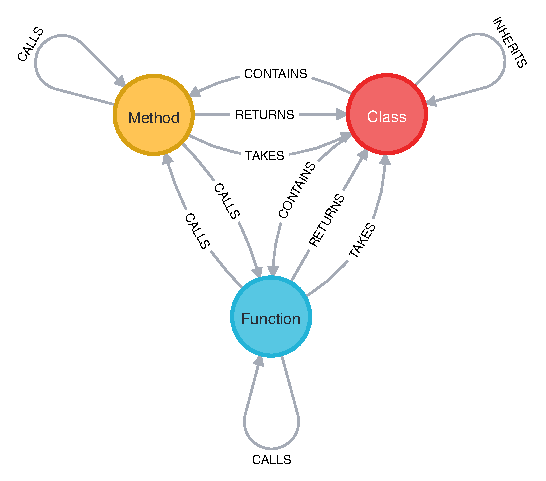
\includegraphics[width=0.4\textwidth]{figures/schema-visualization.eps}
\end{center}
\caption{Neo4j Scheme Visualization (To be updated*)}
\label{fig:schema-vis}
\end{figure}


\subsubsection{Code Smells Detector}
...

\newpage
\newpage
\newpage
\newpage

\section{Evaluation}
\label{sec:eval}

% This section presents the evaluation results verifying the proposed solution and provides data confirming that the objectives are met.  If there is no ``Implementation'' section, this section typically starts with the implementation of the solution here, {\em e.g.}, how each part of the solution is implemented and the tools and software used (with proper reference).  Next, this section should present the evaluation setup, including the computing environments ({\em e.g.}, hardware and software specs where the experiments are deployed), network setting (if involved), any alteration in the implementation, and dataset driving the experiments. The setup is followed by an introduction on comparison algorithms and rationals for choosing them for validating the proposed solution.  Before diving into the evaluation results, it is also important to define all performance metrics and the rational/importance of using them.

% The rest of this section presents the evaluation results that are typically organized into subsections.  The subsections are typically organized in a way that best highlights the advancements brought by the proposed solution and shows the novelty of the work.  

% When presenting results from each experiment, it is important to first explain the purpose of the experiment and parameter setup.  Tables, charts, and plots are typically used to visually present the results.  There are many tools for generateing plots such as {\tt gnuplot} \cite{gnuplot}.  When explaining the results, focus on the insightful observations instead of the obvious results.  The discussion around each experiment should lead to conclusive statements about the correctness of the solution, the advancements, and the novelty.



\begin{table}[h]
\centering
\begin{threeparttable}
\begin{tabular}{|p{2cm}||p{2cm}|p{2cm}|}

\hline
\textbf{Name} & \textbf{Name} & \textbf{Amount} \\
\hline

\multirow{6}{*}{\href{https://github.com/huggingface/transformers}{Transformers}}   
                                & Class  & 8,609 \\ \cline{2-3}
                                & Function  & 24,301 \\ \cline{2-3}
                                & Call  & 22,464 \\ \cline{2-3}
                                & Containment  & 21,611 \\ \cline{2-3}
                                & Inheritance  & 5,659 \\ \cline{2-3}
                                & Return  & 1,142 \\ \cline{2-3}
\hline
\end{tabular}
\caption{Knowledge graph metrics for selected projects}
\label{tab:graph-metrics}
\end{threeparttable}
\end{table}

\section{Conclusion}
\label{sec:conclusion}

% This section concludes the paper with a summary of the work and highlights of advancements. 




\bibliographystyle{ACM-Reference-Format}
\bibliography{main}

\appendix
\section{Libraries \& Tools Used}
\label{sec:appendix-a}

This appendix details the libraries and tools utilized in the development of the codebase parser for converting source code into Knowledge Graphs.

\begin{enumerate}
    \item \textbf{Neo4j (Neo4j, Inc.)} \\
    \textit{Description:} A graph database management system.
    
    \item \textbf{Neomodel (Version 5.2.0)} \\
    \textit{Description:} Object Graph Mapper (OGM) for Python and Neo4j.
    
    \item \textbf{Astroid (Version 3.0.1)} \\
    \textit{Description:} An abstract syntax tree for Python with inference support.
    
    \item \textbf{Mongo DB (MongoDB Inc.)} \\
    \textit{Description:} A source-available, cross-platform, document-oriented database program.
    
    \item \textbf{PyMongo (Version 4.6.1)} \\
    \textit{Description:} Python distribution containing tools for working with MongoDB.
\end{enumerate}



\end{document}
